%\documentclass{article}
%\usepackage[a4paper, total={6in, 8in}]{geometry}
%\documentclass[reprint,amsmath,amssymb,rmp,onecolumn,notitlepage,11pt]{revtex4-1}
\documentclass[notitlepage,
reprint,%twocolumn,
%preprint
onecolumn,
amsmath,amssymb,superscriptaddress,aps,
pre]{revtex4-1}
\usepackage[utf8]{inputenc}
%\usepackage{authblk}
%\usepackage{natbib}
\usepackage[normalem]{ulem}
\usepackage{graphicx}
\usepackage{hyperref}
\usepackage{xcolor}
\newcommand{\red}[1]{\textcolor{red!80!black}{#1}}
\newcommand{\blue}[1]{\textcolor{blue!80!black}{#1}}
\newcommand{\green}[1]{\textcolor{green!70!black}{#1}}
\newcommand{\gray}[1]{\textcolor{gray!80!black}{#1}}
\usepackage{mathtools}
\DeclarePairedDelimiter{\evdel}{\langle}{\rangle}
\usepackage[colorinlistoftodos]{todonotes}
\newcommand{\Pin}{P_{\mathrm{in}}}
\newcommand{\fhigh}{f_{\mathrm{high}}}
\newcommand{\flow}{f_{\mathrm{low}}}
\setlength {\marginparwidth }{2cm}


\begin{document}
\title{Supplementary material accompanying "Theory of chain separation distributions gives insights in real protein contact networks"}
\author{Nora Molkenthin}
\affiliation{Potsdam Institut für Klimafolgenforschung}
\affiliation{Center for Advancing Electronics Dresden (cfaed), Technical University of Dresden}
\author{J. J.  Güven}
\affiliation{EaStCHEM School of Chemistry, University of Edinburgh, Edinburgh, United Kingdom}
\author{Steffen Mühle}
\affiliation{Uni Göttingen, 37077 Göttingen, Germany}
\author{Antonia S J S Mey}
\email[Electronic Address: ]{antonia.mey@ed.ac.uk}
\affiliation{EaStCHEM School of Chemistry, University of Edinburgh, Edinburgh, United Kingdom}
\maketitle

\section*{Optimizing theory parameters}

 Fig.~\ref{fig:2d} shows a grid of the two-dimensional simulations for amino acid distance distributions for chains of around 498 amino acids long. The solid line shows the theoretical distribution given in Eq.~(12) of the main article. Each column corresponds to a different value of the scaling parameter $A$ and each row to a different value of the exponent parameter $a$ for this theoretical distribution. Plotted also is the 95\% confidence level for the 2D amino acid distance distribution. 

In addition to plotting this amino acid distance distribution grid, we also plotted the residual plots for each combination of parameters. These are shown in Fig.~\ref{fig:2d_r}. The residual sum of squares $\Sigma \sigma$, $R^2$ statistic and mean of residuals, $\bar{\sigma}$, were calculated for each combination of parameters $a$ and $A$. 

The choice of parameters was first narrowed down by looking at how well the theoretical distribution appeared to fit the amino acid distance distribution of the simulations in Fig.~\ref{fig:2d}, as well as the spread of residuals around the theoretical line in Fig.~\ref{fig:2d_r}. From Fig.~\ref{fig:2d}, we chose a smaller group of plots where the theoretical distribution fitted through a majority of simulation data points. Similarly, from Fig.~\ref{fig:2d_r}, we chose a group of plots where the majority of residuals were randomly scattered around zero. The non-linear parts of the residuals both at the low and high ends of the amino acid distances were expected from Fig.~\ref{fig:2d}. In the next step, we found the optimal parameters by finding the best combination of statistics, i.e. a minimized residual sum of squares, $\Sigma \sigma^2$, maximized constant of determination, $R^2$ and the mean of residuals, $\bar{\sigma} \approx 0$. This was done to avoid relying on a single statistic to determine the optimal parameters. For this 2D simulation data, we chose $A=0.39$ and $a=6$, which produced the following statistics: $\Sigma \sigma^2 = 17.4\times10^3$, $R^2 = 90.0$~\% and $\bar{\sigma} = -0.265$.

The above steps were repeated for both the AlphaFold 2 and RCSB PDBs, for each chain length range. Tables~\ref{table:af}~and~\ref{table:rcsb} show the optimized parameters and their statistics for PDBs obtained from AlphaFold 2 and RCSB, respectively. Figs.~\ref{fig:AF100},~\ref{fig:AF200}~and~\ref{fig:AF300} show the parameter grid plots of amino acid distance distributions for chains of 100, 200 and 300 amino acids long, respectively. Similarly, Figs.~\ref{fig:AF100_r},~\ref{fig:AF200_r}~and~\ref{fig:AF300_r} show the residual plots. While the 95\% confidence intervals are plotted for the PDBs, these were not plotted in the main article for clarity, as the confidence level appears smaller than the scatter markers. 

\begin{table}[tb]
\centering
\begin{tabular}{|c c c c c c|}
\hline
Chain length  & $A$ ($10^{-3}$) & $a$ & $\Sigma \sigma^{2}$ & $R^2$ (\%) & $\bar{\sigma}$ \\
\hline
100 & 2.1 & 3 & 0.0002 & 57 & 0.0001 \\
200 & 1.1 & 3 & 0.0135 & 62 & -0.0005 \\
300 &1.0 & 5 & 0.1478 & 76  & -0.0012 \\
\hline
\end{tabular}
 \caption{Detailed parameters and statistics for PDBs obtained from AlphaFold 2. Shown are the optimized parameters $A$ and $a$ used to fit the theoretical amino acid distance distribution given in Eq.(12) of the main article, for chains of 100, 200 and 300 amino acids long.  Shown also are the residual sum of squares ($\Sigma \sigma^{2}$), constant of determination ($R^2$) and the mean of residuals ($\bar{\sigma}$) for each fit.}
\label{table:af}
\end{table}

\begin{table}[h]
\centering
\begin{tabular}{|c c c c c c|}
\hline
Chain length & $A$ ($10^{-3}$) & $a$ & $\Sigma \sigma^{2}$ & $R^2$ (\%) & $\bar{\sigma}$ \\
\hline
100 & 1.9 & 2 & 0.0002 & 59 & 0.0001 \\
200 & 1.2 & 3 & 0.0474 & 70 & -0.0010\\
300 & 0.9 & 4 & 0.1102 & 76 & -0.0011\\
\hline
\end{tabular}
 \caption{Detailed parameters and statistics for PDBs obtained from RCSB. Shown are the optimized parameters $A$ and $a$ used to fit the theoretical amino acid distance distribution given in Eq.(12) of the main article, for chains of 100, 200 and 300 amino acids long. Shown also are the residual sum of squares ($\Sigma \sigma^{2}$), constant of determination ($R^2$) and the mean of residuals ($\bar{\sigma}$) for each fit.}
\label{table:rcsb}
\end{table}


\begin{figure*}[htb]
    \centering{
    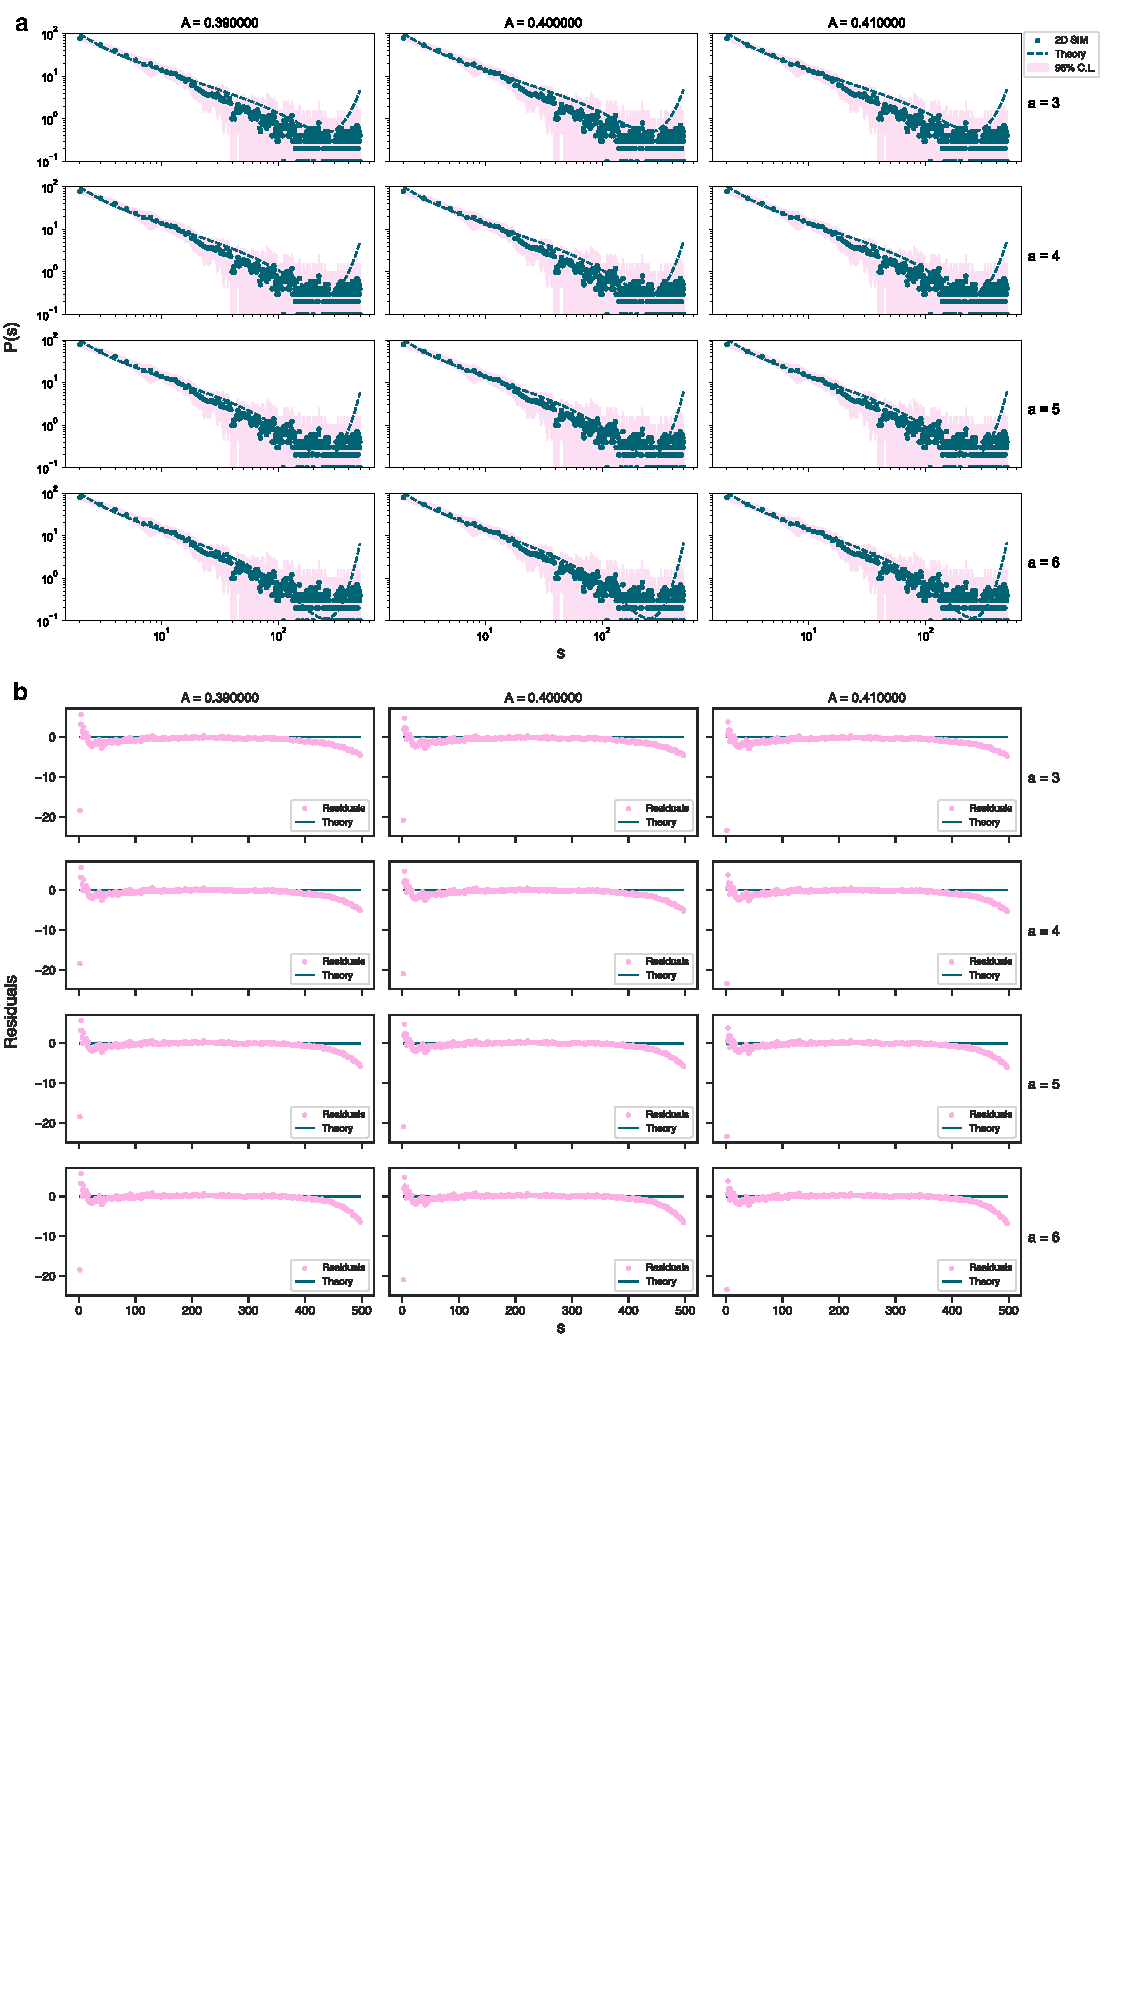
\includegraphics[scale=0.65]{paper/figures/SM_figures/Fig1/Fig1.pdf}
    \caption{a) A grid of the amino acid distance distribution in protein chains of 498 residues long in two-dimensional simulations. The solid line shows the theoretical distribution for different values of parameters $a$ and $A$. b) The residual plots of the amino acid distance distribution around the theoretical distribution. The residual sum of squares, $\Sigma \sigma$, $R^2$ statistic and the mean of residuals, $\bar{\sigma}$, were calculated for each combination of parameters.}
    \label{fig:2d}}
\end{figure*}

\begin{figure*}[htb]
    \centering{
    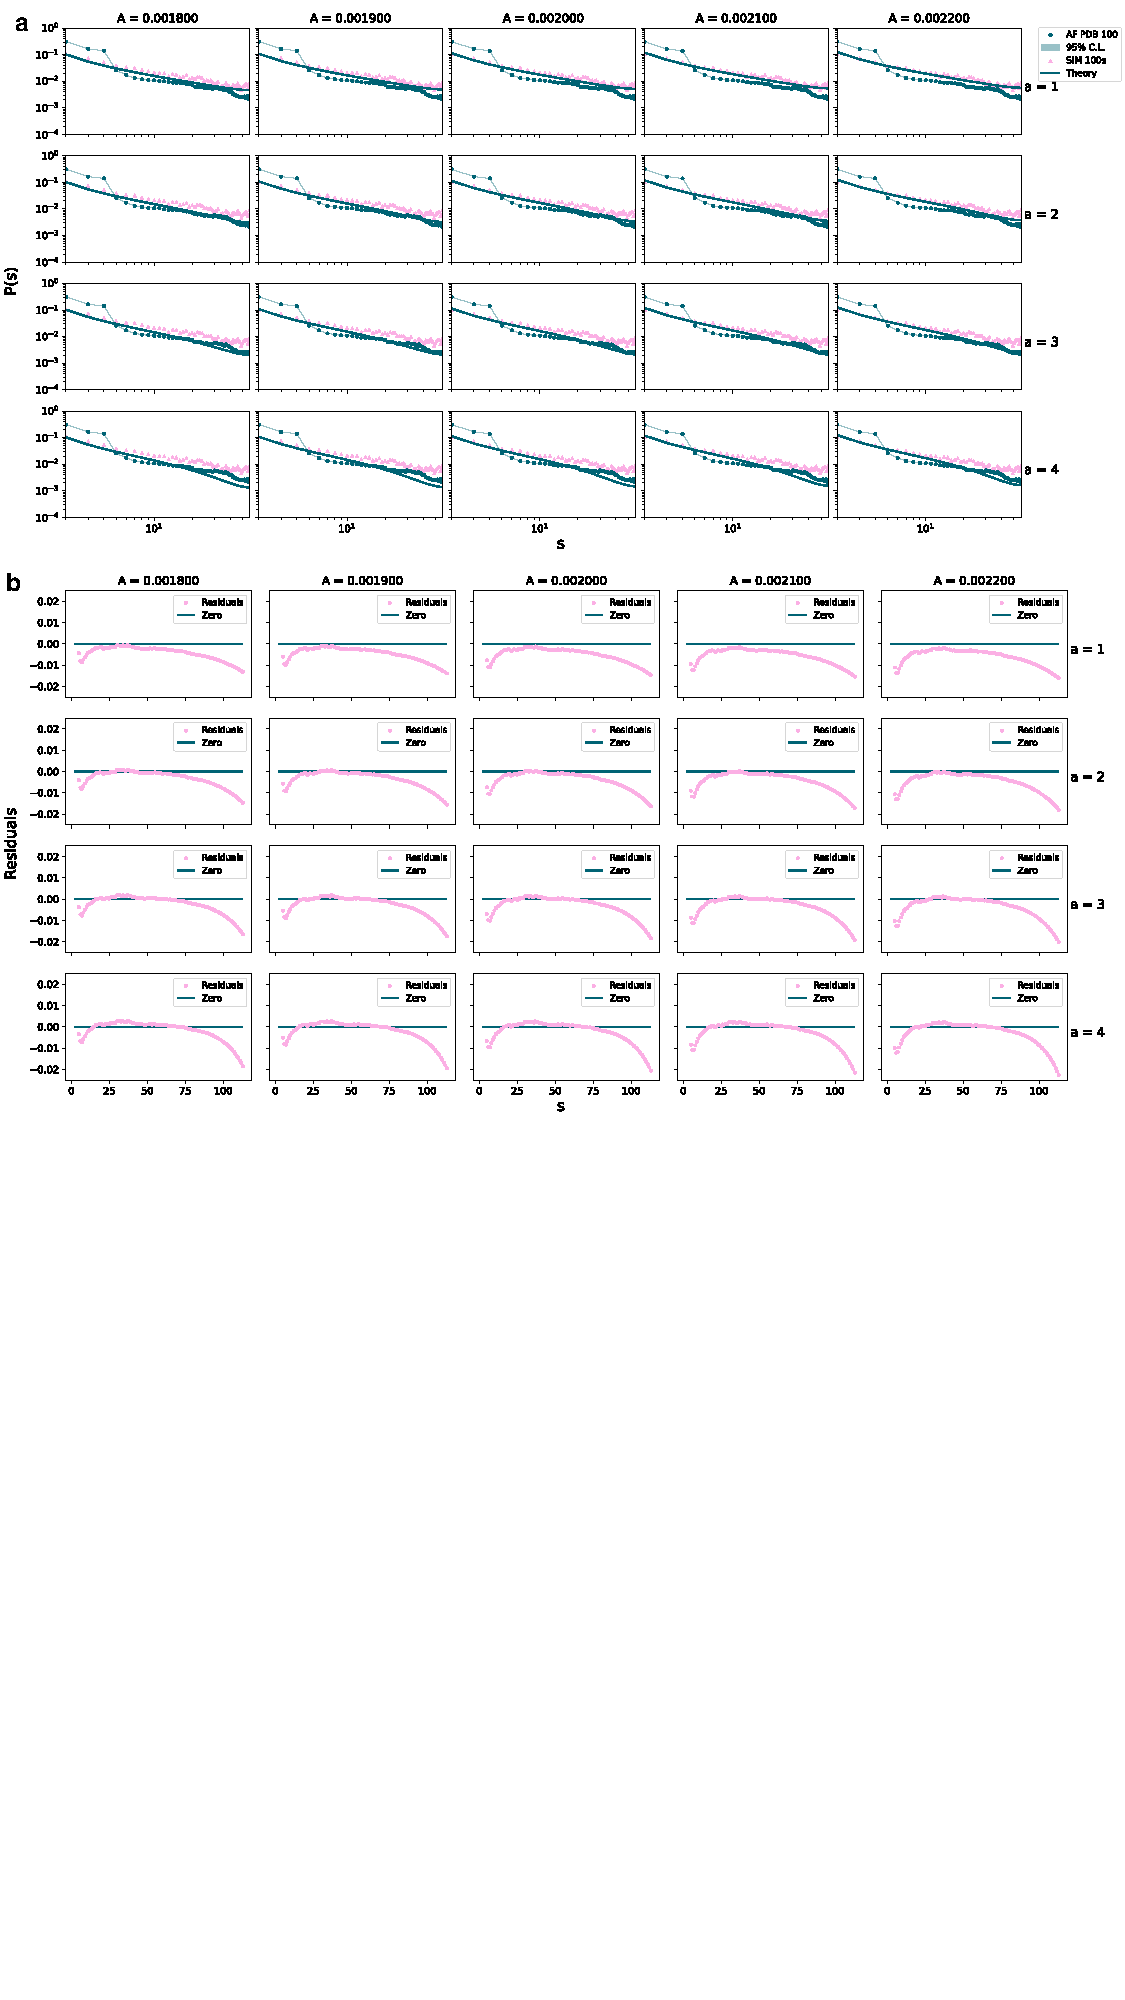
\includegraphics[width=0.8\textwidth]{paper/figures/SM_figures/Fig2/Fig2.pdf}
    \caption{a) A grid of the amino acid distance distributions in chains of around 100 residues long in PDBs obtained from AlphaFold 2. The solid line shows the theoretical distribution for different values of parameters $a$ and $A$. b) The residual plots of the amino acid distance distribution around the theoretical distribution. The residual sum of squares, $\Sigma \sigma$, $R^2$ statistic and the mean of residuals, $\bar{\sigma}$, were calculated for each combination of parameters.}
    \label{fig:AF100}}
    
\end{figure*}

\begin{figure*}[htb]
    \centering{
    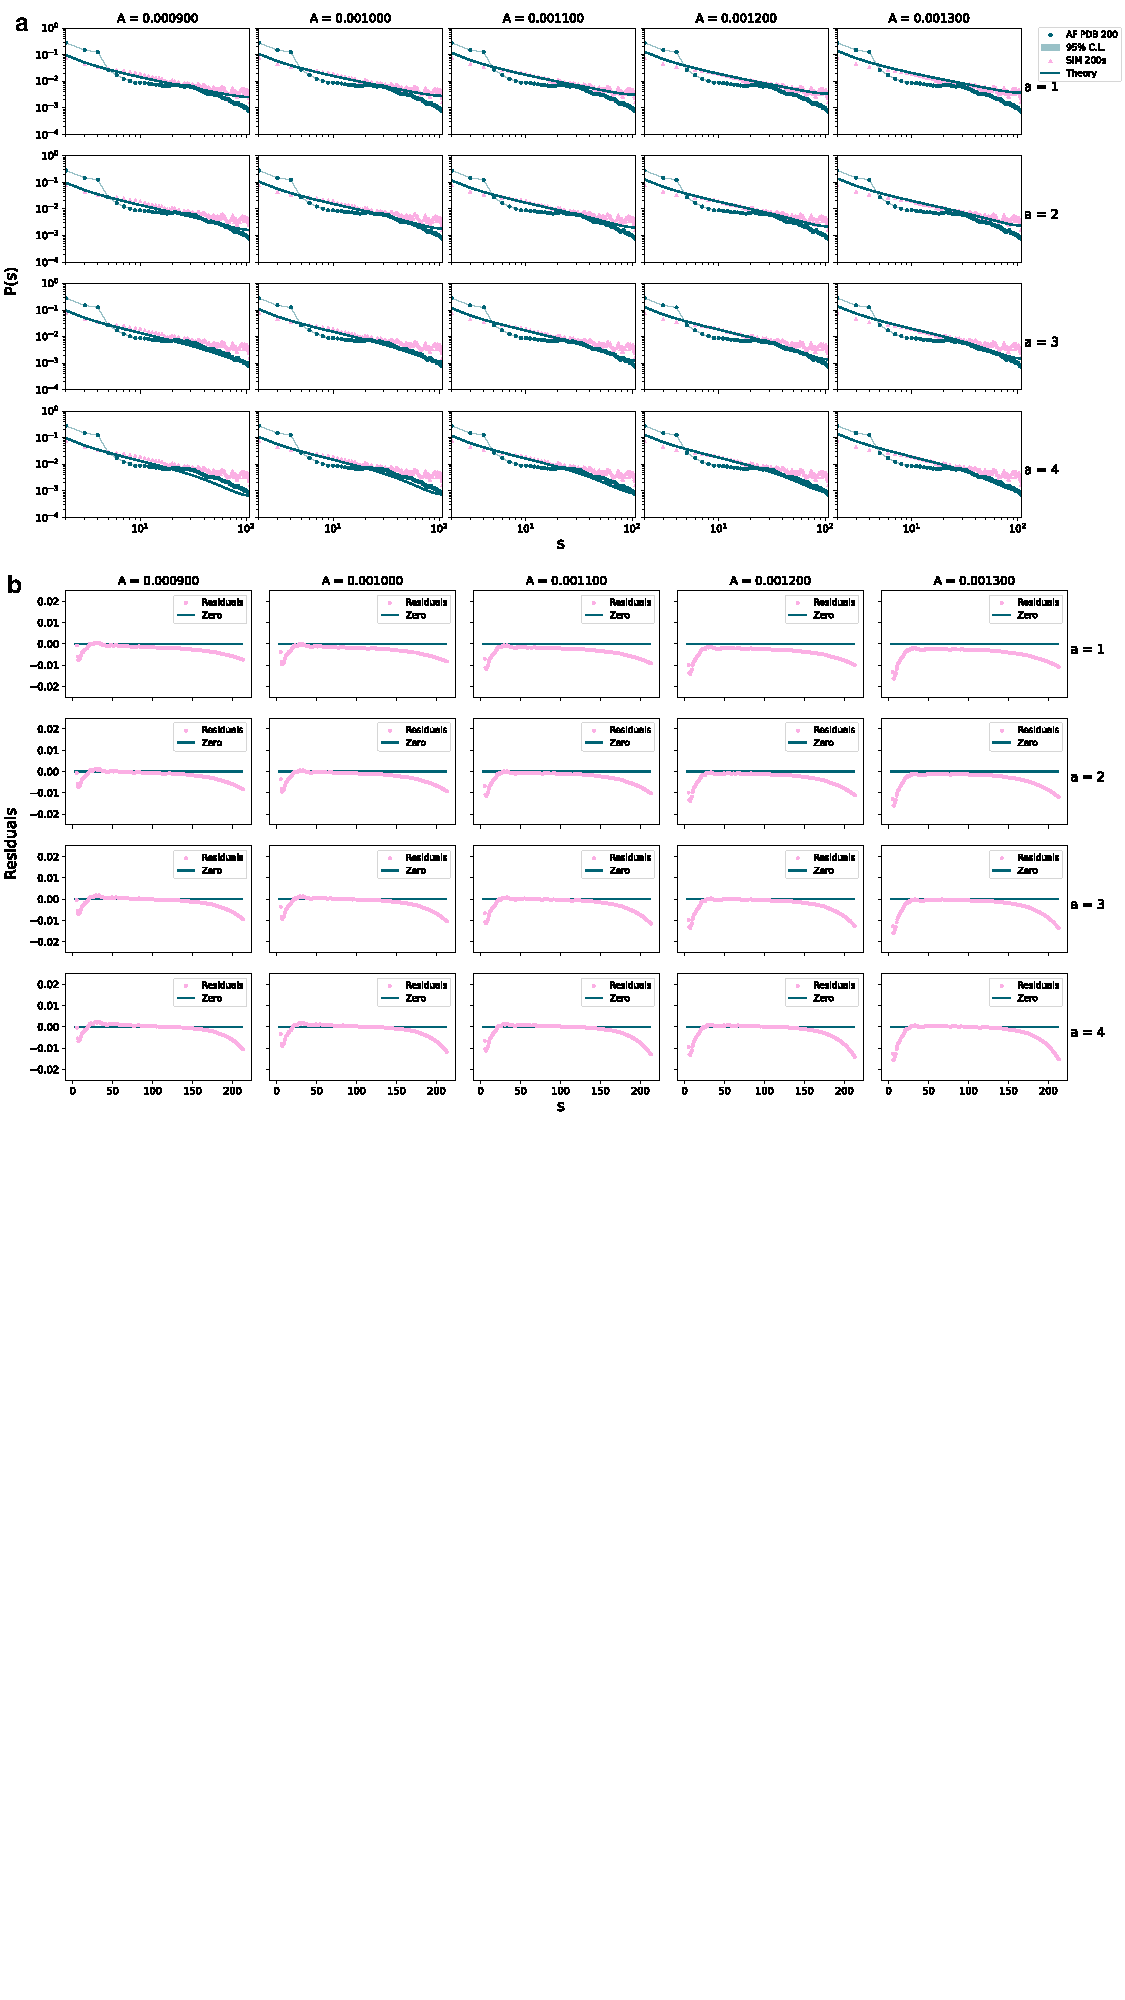
\includegraphics[width=0.8\textwidth]{paper/figures/SM_figures/Fig3/Fig3.pdf}
    \caption{a) A grid of the amino acid distance distributions in chains of around 200 residues long in PDBs obtained from AlphaFold 2. The solid line shows the theoretical distribution for different values of parameters $a$ and $A$. b) The residual plots of the amino acid distance distributions around the theoretical distribution. The residual sum of squares, $\Sigma \sigma$, $R^2$ statistic and the mean of residuals, $\bar{\sigma}$, were calculated for each combination of parameters.}
    \label{fig:AF200}}
\end{figure*}

\begin{figure*}[htb]
    \centering{
    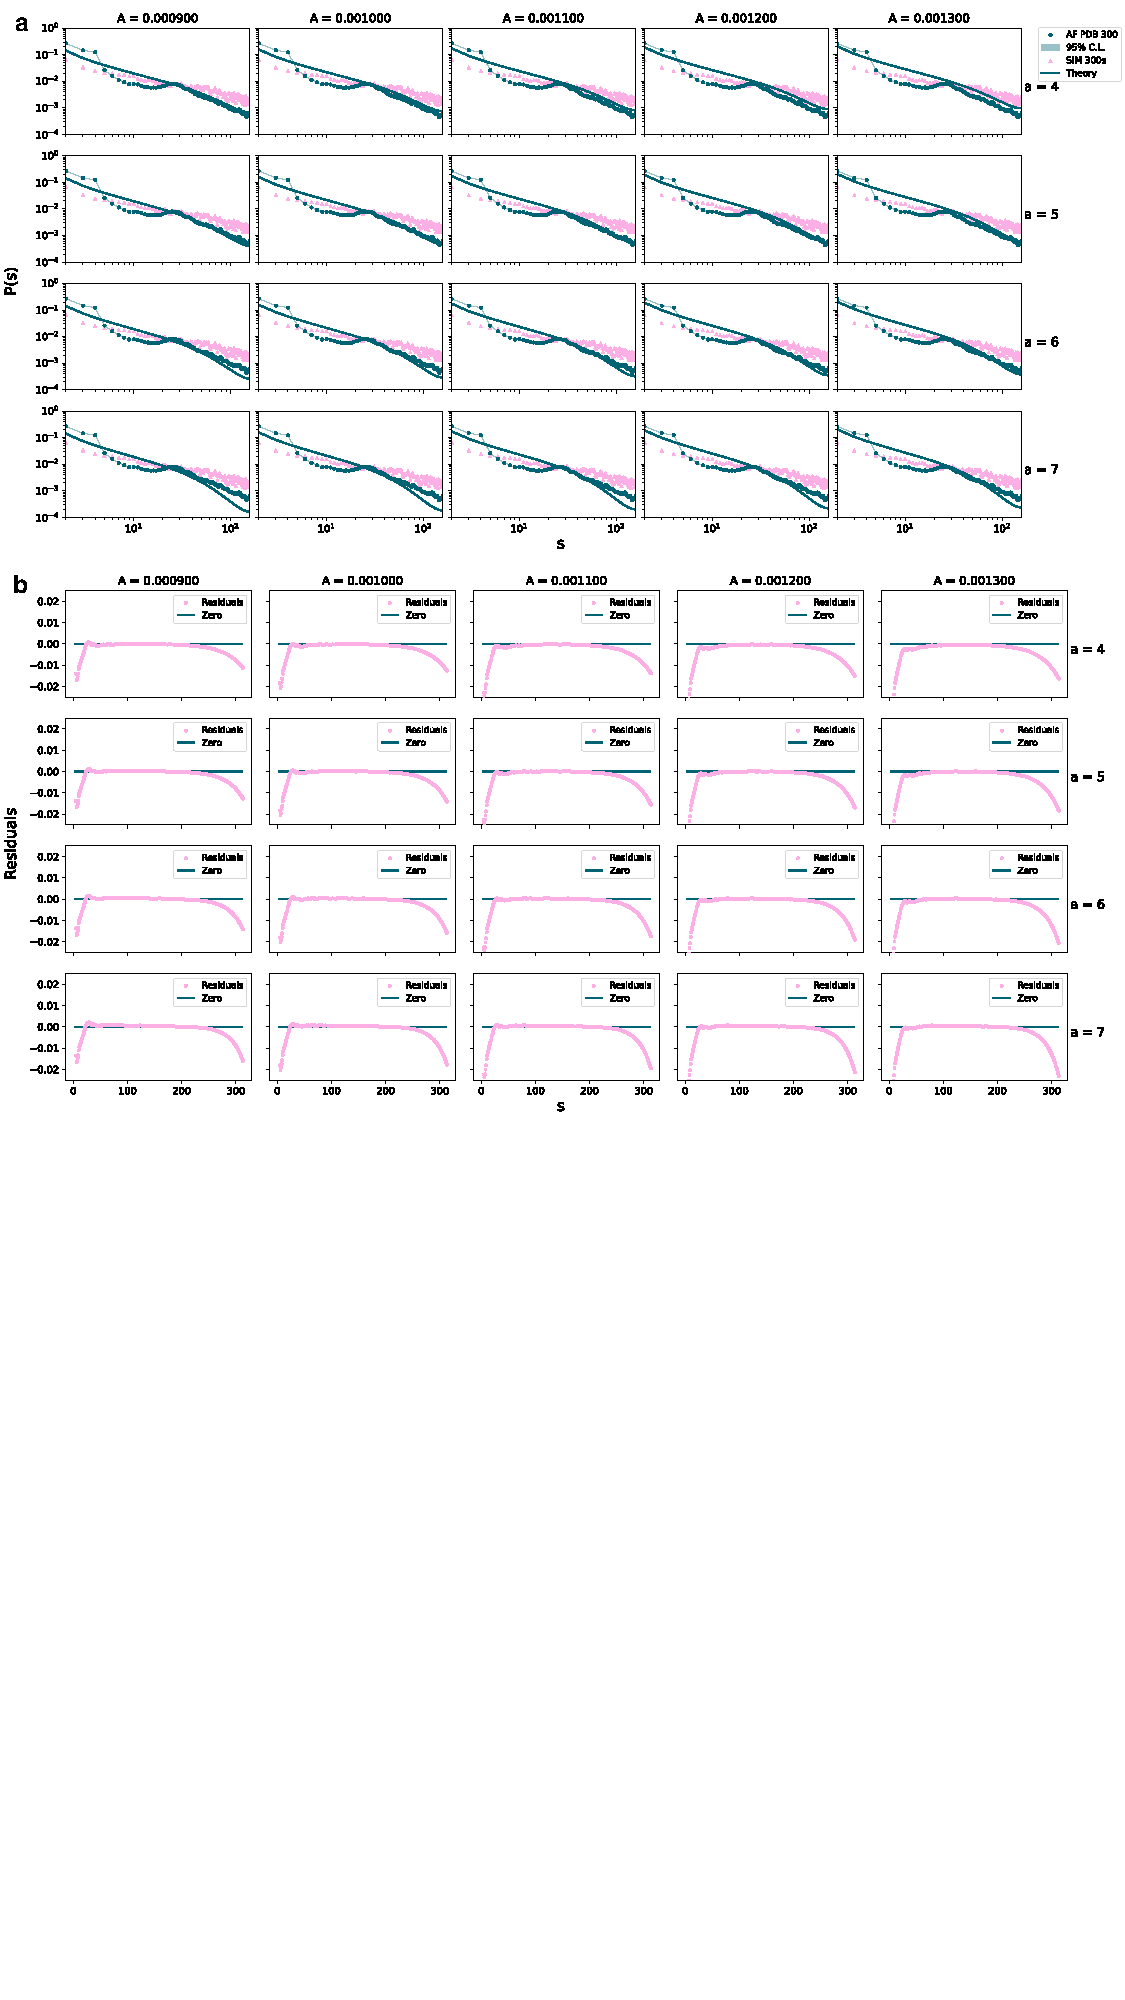
\includegraphics[width=0.8\textwidth]{paper/figures/SM_figures/Fig4/Fig4.pdf}
    \caption{a) A grid of the distribution of link lengths in chains of around 300 residues long in PDBs obtained from AlphaFold 2. The solid line shows the theoretical distribution for different values of parameters $a$ and $A$. b) The residual plots of the amino acid distance distributions around the theoretical distribution. The residual sum of squares, $\Sigma \sigma$, $R^2$ statistic and the mean of residuals, $\bar{\sigma}$, were calculated for each combination of parameters.}
    \label{fig:AF300}}
    
\end{figure*}


\begin{figure*}[htb]
    \centering{
    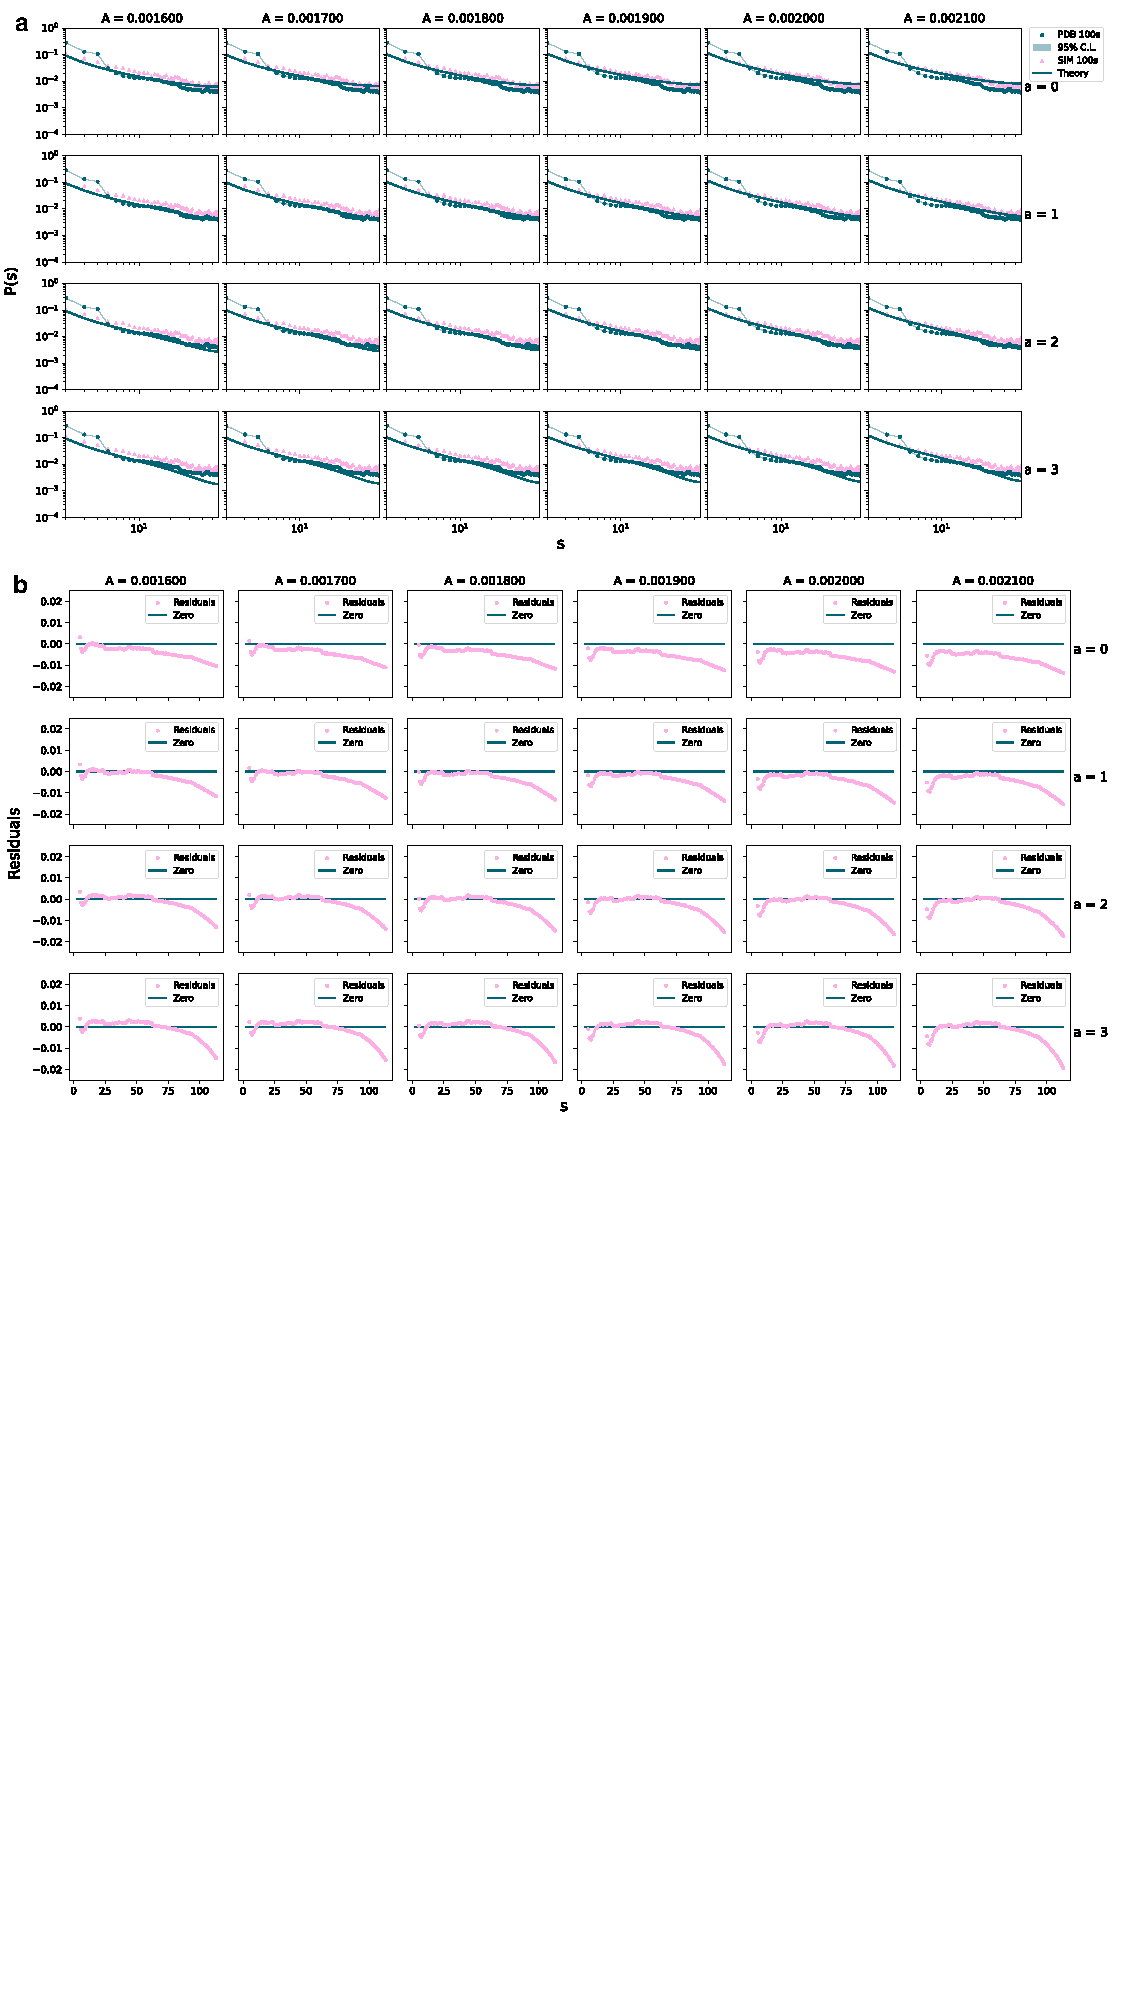
\includegraphics[width=0.8\textwidth]{paper/figures/SM_figures/Fig5/Fig5.pdf}
    \caption{a) A grid of the distribution of link lengths in chains of around 100 residues long in PDBs obtained from RCSB. The solid line shows the theoretical distribution for different values of parameters $a$ and $A$. b) The residual plots of the amino acid distance distributions around the theoretical distribution. The residual sum of squares, $\Sigma \sigma$, $R^2$ statistic and the mean of residuals, $\bar{\sigma}$, were calculated for each combination of parameters.}
    \label{fig:PDB100}}
\end{figure*}

\begin{figure*}[htb]
    \centering{
    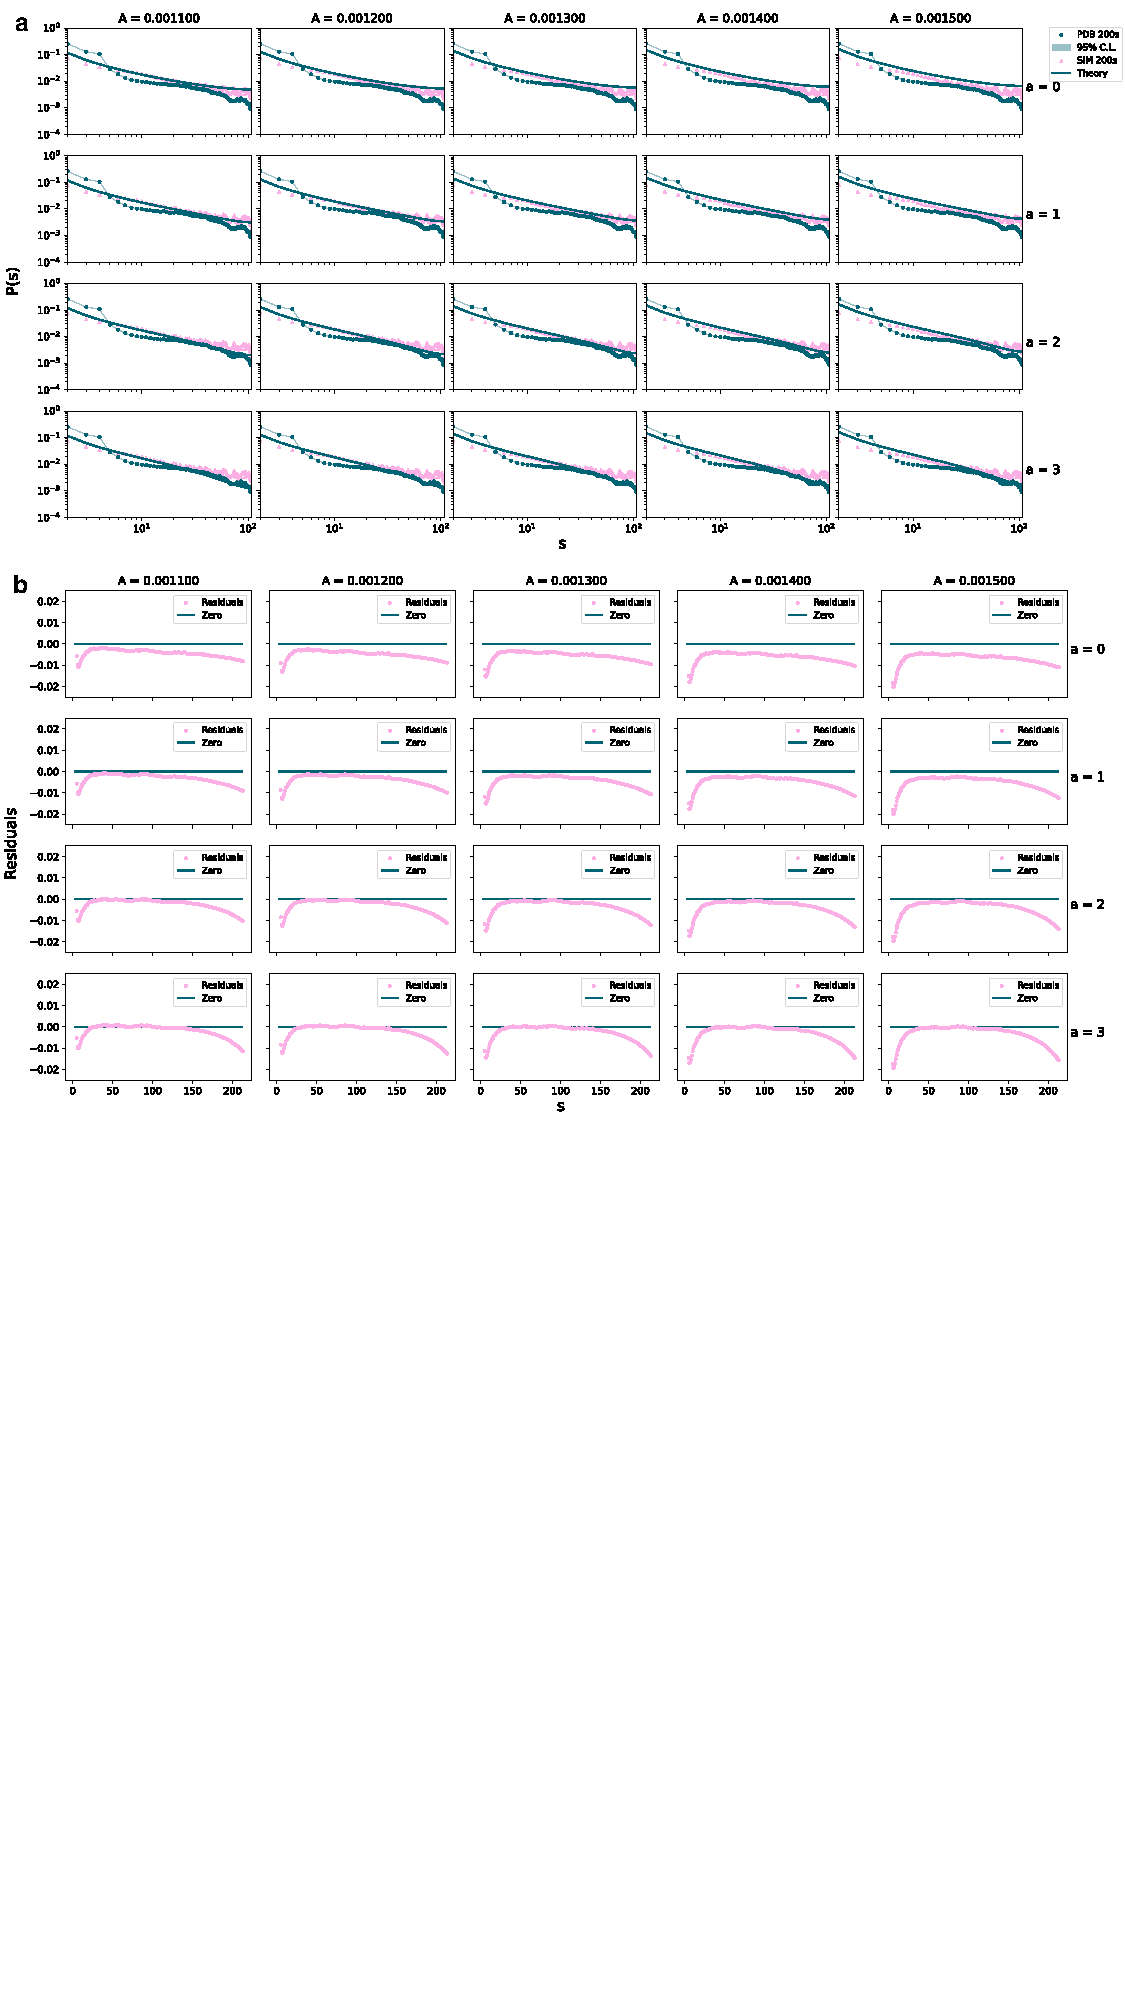
\includegraphics[width=0.8\textwidth]{paper/figures/SM_figures/Fig6/Fig6.pdf}
    \caption{A grid of the distribution of link lengths in chains of around 200 residues long in PDBs obtained from RCSB. The solid line shows the theoretical distribution for different values of parameters $a$ and $A$. b) The residual plots of the amino acid distance distributions around the theoretical distribution. The residual sum of squares, $\Sigma \sigma$, $R^2$ statistic and the mean of residuals, $\bar{\sigma}$, were calculated for each combination of parameters.}
    \label{fig:PDB200}}
    
\end{figure*}

\begin{figure*}[htb]
    \centering{
    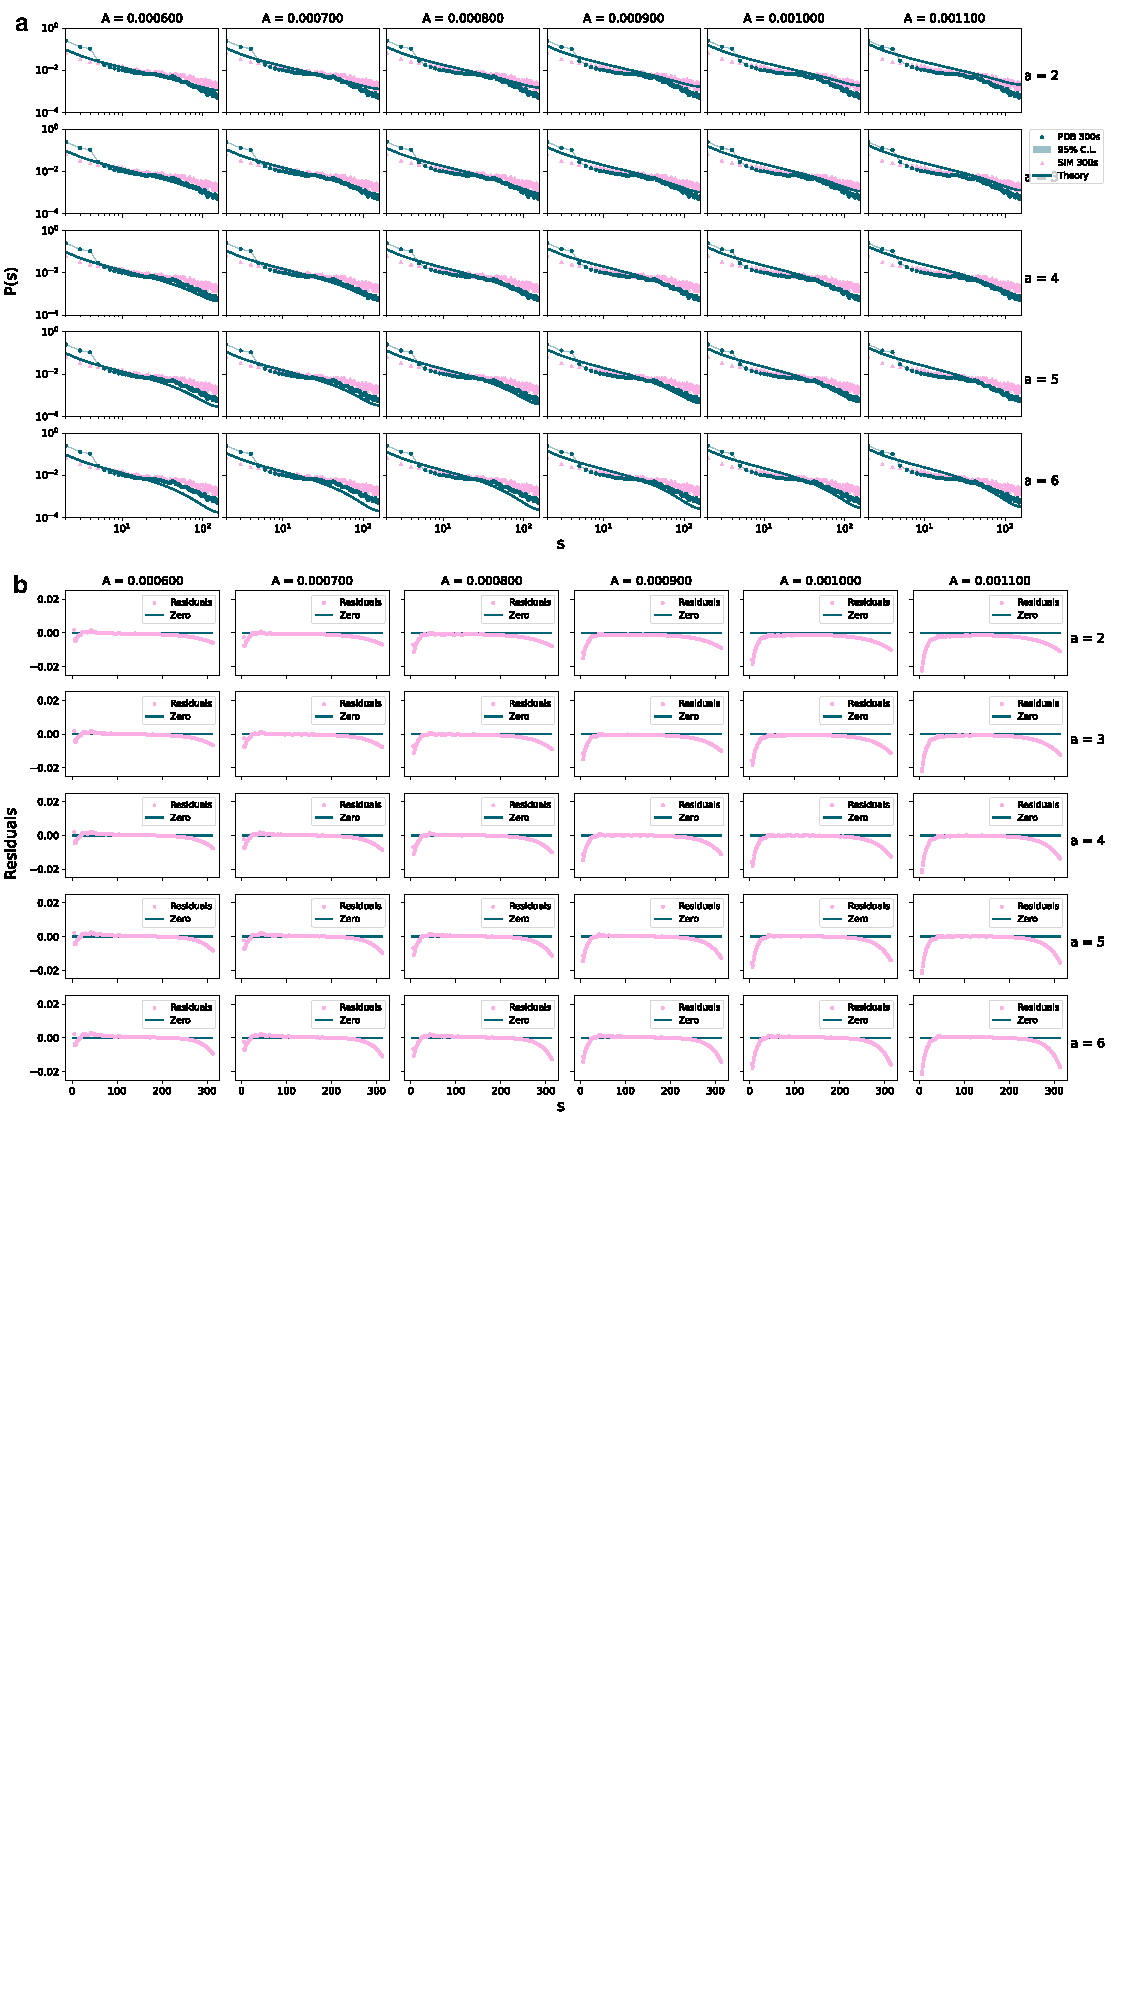
\includegraphics[width=0.8\textwidth]{paper/figures/SM_figures/Fig7/Fig7.pdf}
    \caption{A grid of the distribution of link lengths in chains of around 300 residues long in PDBs obtained from RCSB. The solid line shows the theoretical distribution for different values of parameters $a$ and $A$. b) The residual plots of the amino acid distance distributions around the theoretical distribution. The residual sum of squares, $\Sigma \sigma$, $R^2$ statistic and the mean of residuals, $\bar{\sigma}$, were calculated for each combination of parameters.}
    \label{fig:PDB300}}
\end{figure*}


\bibliographystyle{unsrt}
% \bibliography{proteins}

\end{document}